\chapter{Ajouter une table à la base de données}

\section{Définir une nouvelle table}

Afin d'ajouter une nouvelle table dans la base de données, il est nécessaire de modifier le fichier models.py présent dans le dossier tennis (Figure~\ref{}). Pour ce faire, il suffit d'ouvrir le fichier à l'aide d'un éditeur de code (Notepad, Pycharm, etc.), et de rajouter une nouvelle classe à la fin de celui-ci en respectant l'indentation et la syntaxe python appropriée. La structure d'une classe est définie sur la figure~\ref{fig:Structure d'une classe représentant une table de la base de données}

\begin{figure}[!ht]
\centering
\begin{framed}
\lstinputlisting[language=Python, firstline=1, lastline=8]{"developer_guide/class.py"}
\end{framed}
\caption{Structure d'une classe représentant une table de la base de données}
\label{fig:Structure d'une classe représentant une table de la base de données}
\end{figure}
\FloatBarrier

Cette structure se complète ensuite en définissant l'ensemble des variables de classe (représentant les différentes informations à stocker dans la base de données) en spécifiant leurs types et leurs éventuelles relations et en y complétant les méthodes \textit{str} et \textit{unicode}. On peut observer un exemple d'une telle classe sur la figure~\ref{fig:Classe issue du fichier models.py représentant une table de la base de données}

\section{Les types de champs possibles}

La définition du type de chaque champ de la table se fait par des appels à des fonctions spécifiques. Les principales fonctions sont les suivantes :\\

\begin{itemize}
\item \textit{models.CharField()} : définit un champ contenant une chaine de caractères
\item \textit{models.AutoField()} : définit un champ contenant un entier se remplissant de manière automatique et incrémentale en fonction des identifiants disponibles
\item \textit{models.BooleanField()} : définit un champ contenant un booléen (True ou False)
\item \textit{models.DecimalField()} : définit un champ contenant un nombre décimal de taille fixe
\item \textit{models.DateTimeField()} : définit un champ contenant une date et une heure
\item \textit{models.TextField()} : définit un champ contenant une chaine de caractère (de très grande taille)\\
\end{itemize}

En plus de fournir un type à chaque champ, il est également possible de les paramétrer (valeur par défaut, degré d'obligation du champ, éditable ou non, etc.) en précisant divers arguments aux différents appels de fonctions définis précédemment. Ces arguments sont définis dans la documentation Django disponible à l'adresse suivante: \url{https://docs.djangoproject.com/fr/1.9/ref/models/fields/}\\

La définition des relations entre les tables se fait de manière semblable à la définition du type d'un champ. Ces relations sont spécifiées via des appels à des fonctions, applicables à un champ particulier. Les relations principales entre les différents champs sont les suivantes :\\

\begin{itemize}
\item \textit{models.ForeignKey()} : définit une relation plusieurs-à-un (One to many)
\item \textit{models.OneToOneField()} : définit une relation un-à-un (One to one)
\item \textit{models.ManyToManyField()} : définit une relation plusieurs à plusieurs (Many to many)\\
\end{itemize}

De même que pour les fonctions définissant le type d'un champ, il est également possible de définir plusieurs paramètres passés en arguments lors de la création des relations  (comme le nom à utiliser pour la relation inverse depuis l’objet lié vers celui-ci, si le champ est obligatoire ou non, etc.)\\

\begin{figure}[!ht]
\centering
\begin{framed}
\lstinputlisting[language=Python, firstline=9, lastline=24]{"developer_guide/class.py"}
\end{framed}
\caption{Classe issue du fichier \textit{models.py} représentant une table de la base de données}
\label{fig:Classe issue du fichier models.py représentant une table de la base de données}
\end{figure}
\FloatBarrier

\section{Mettre à jour la base de données}

Une fois terminé, il ne reste qu'à sauvegarder les modifications apportées au fichier, le fermer, et effectuer la migration de la base de données (afin que ceux-ci soient bien effectués) grâce aux commandes (dans cet ordre) : python manage.py makemigrations et python manage.py migrate. Un nouveau fichier contenant les modifications apportées à la base de données sera créé dans le dossier ASMAE/tennis/migrations, ce qui permet d'avoir une vue d'ensemble de l'évolution de la base de données mais surtout de pouvoir effectuer des restaurations à des versions antérieures (rollbacks) si besoin est.\\


L'ensemble de la documentation se rapportant aux commandes de migration de la base de données est disponible à l'adresse suivante : https://docs.djangoproject.com/en/1.9/topics/migrations/.\\

Une fois la migration effectuée, il est possible de directement aller vérifier sur la nouvelle table a correctement été ajoutée, ou si la ou les modifications ont bien été apportées à la base de données via l'interface administration de Django. Il suffit pour cela de se connecter à l'adresse du site web suivi de "/admin" avec les identifiants d'administrateur, et de se rendre dans l'onglet "Tennis".\\

\begin{figure}[H]
\centering
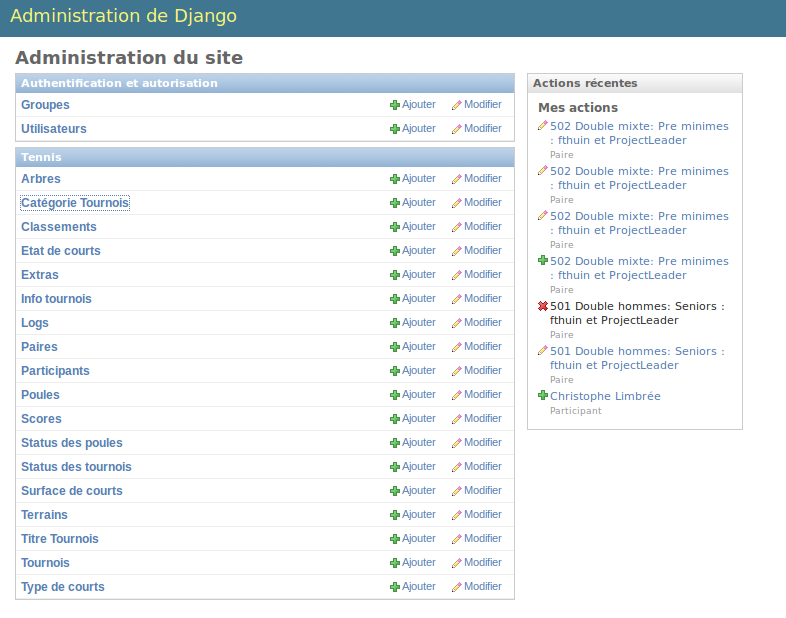
\includegraphics[scale=0.4]{Admin.png}
\caption{Interface administrateur}
\end{figure}

Il est intéressant de noter que la même démarche peut être suivie lorsqu'une ou plusieurs modifications doivent être apportées à une table déjà existante dans la base de données.\\

Ajouter une view et template correspondant :\\

Afin de rajouter du nouveau contenu sur le site internet, il est utile de pouvoir créer de nouvelles pages, et de les rendre accessibles à partir de celles déjà présentes.\\

Pour ce faire, il faut dans un premier temps créer le template, c'est à dire la structure de la page en HTML. Une fois le fichier représentant la page créé, il faut l'ajouter au dossier contenant l'ensemble des pages HTML du site, c'est-à-dire "ASMAE/tennis/templates". Il est intéressant de noter que les différents éléments statiques (tels qu'un style css, police particulière, ...) doivent être ajoutés dans le sous-dossier correspondant, présent dans le répertoire "ASMAE/tennis/static/tennis".\\

\begin{figure}[H]
\centering
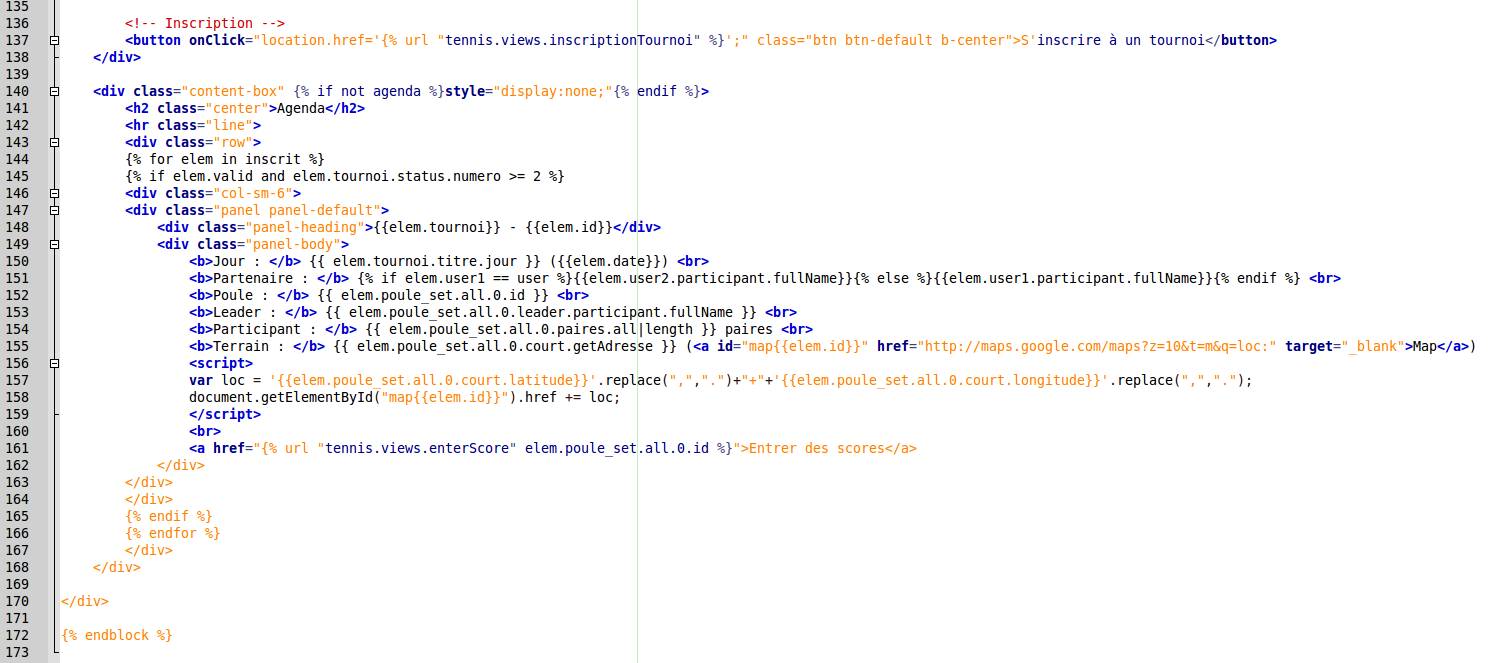
\includegraphics[scale=0.3]{html.png}
\caption{Exemple d'une page HTML}
\end{figure}

Une fois fait, il est nécessaire de créer une view dans le fichier views.py se trouvant dans le dossier "ASMAE/tennis", qui reprendra la page à renvoyer quand un utilisateur fera une requête pour obtenir la page. Le format le plus classique et simpliste d'une telle requête est le suivant: on définit le nom de la requête, ainsi que la page à rendre quand celle-ci est effectuée.\\

\begin{figure}[H]
\centering
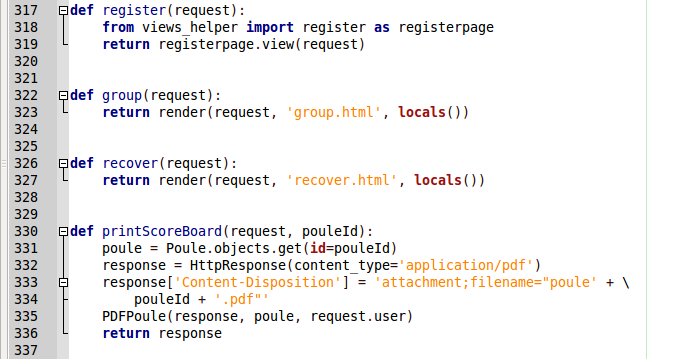
\includegraphics[scale=0.4]{views.png}
\caption{Fichier views.py}
\end{figure}

Enfin, il reste à ajouter au fichier urls.py (également présent dans le dossier "ASMAE/tennis") qui contient tous les liens URL disponibles sur le site, ainsi que le lien vers le nom des views concernées. Pour ce faire, il suffit de rajouter une nouvelle ligne dans le fichier, en respectant le format suivant : url(NouveauLienUrl, NomDeLaViews), .

\begin{figure}[H]
\centering
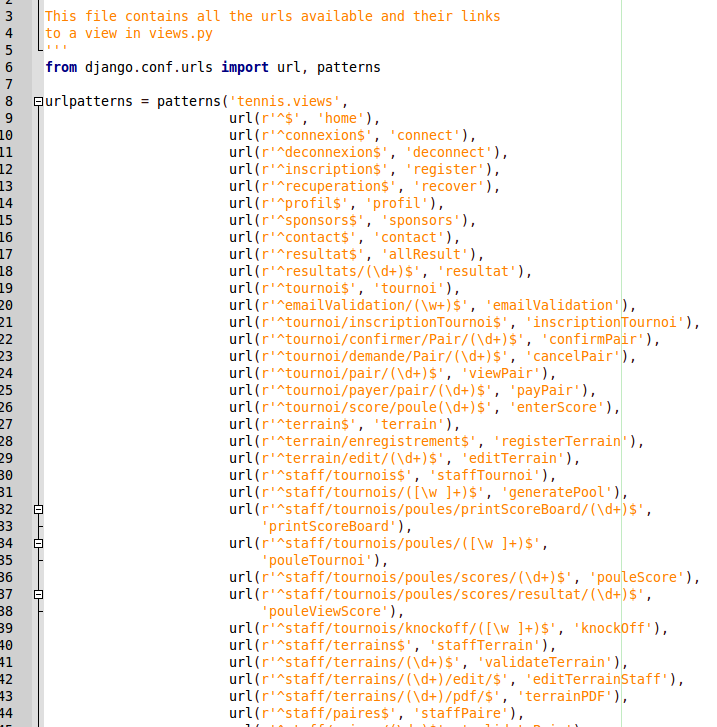
\includegraphics[scale=0.4]{url.png}
\caption{Fichier urls.py}
\end{figure}
